\section{Unification}
Dans notre cas, nous nous intéressons à l'unification \textit{higher order}, à l'opposition de l'unification \textit{first order} étudiée par Robinson en 1965 \cite{robinson1965machine}\cite{robinson1971computational}. Nous avons trouvé 2 implémentations possibles que nous avons essayé de mettre en place : 
\begin{itemize}
    \item Dowek
    \item Huet
\end{itemize}

\subsection{Algorithme de Dowek}

\subsubsection{Precooking}

En $\lambda\sigma$-calcul, les opérations grafting et de réduction commutent. C'est pour cette raison que l'on peut utiliser le grafting dans l'unification higher-order du \lsc{}. En effet l'unification dans le \lsc{} calcule un grafting qui rends les termes égaux, tandis que l'unification dans le lambda-calcul calcule une substitution. Pour réaliser l'unification higher-order, on souhaite travailler avec des graftings.

Pour réaliser l'unification dans le \lc{}, on va traduire les termes du \lc{} vers le \lsc{}, cette opération est nommée precooking :

\begin{defn}
Soit $a \in \Lambda_{DB}(X)$ tel que $\Gamma \vdash a\ :\ T$. Pour chaque variable $X$ de type $U$ dans le terme $a$, on associe le type $U$ dans le contexte $\Gamma$ dans le \lsc{}. Le precooking de $a$ depuis le \lc{} vers le \lsc{} est défini par $a_F = F(a, 0)$ où $F(a, n)$ est :

\begin{enumerate}
    \item $F((\lambda_B a), n) = \lambda_B(F(a, n + 1))$
    \item $F(k, n) = 1[\uparrow^{k-1}]$
    \item $F((a b), n) = F(a, n) F(b, n)$
    \item $F(X, n) = X[\uparrow^n]$
\end{enumerate}

\end{defn}

\subsubsection{Algorithme d'unification}

Nous allons présenter l'algorithme d'unification utilisé dans le papier de Dowek \cite{dowek1995higher}. Comme dit précédemment, une solution est un grafting des métavariables vers les termes.

D'un point de vus formelle on cherche à appliquer des règles d'unification (présentées \hyperref[unificationrules]{plus tard}) sur un système d'équations. Nous avons dû faire un choix afin de représenter cela dans notre système. Voici les différentes structures que nous avons définies :

\begin{lstlisting}
type equa = 
  | DecEq of s_term * s_term
  | Exp

type and_list = equa list

type unif_rules_ret =
  | Ret of (and_list * meta_var_str) list
  | Rep of name * s_term * and_list
  | Nope
  | Fail
\end{lstlisting}

Le type \verb|equa| permet de représenter les équations. Nous avons besoin d'un cas \verb|exp| qui sera utilisé par notre fonction d'unification pour traiter le cas où il n'y a plus aucunes équations sur lesquelles appliquer des règles, nous y reviendrons plus tard.

Le type \verb|and_list| nous permet de représenter les 
disjonctions du système d'équations.
Et enfin le type \verb|unif_rules_ret| est notre type de retour personnalisé pour l'algorithme d'unification.
Avant d'expliquer ce type, il est important de parler de l'architecture des fonctions que nous avons définies pour l'unification.
\begin{figure}[H]
    \centering
    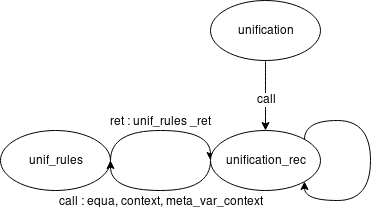
\includegraphics[scale=0.6]{images/unif_diagram.png}
\end{figure}

Étant donné que certaines règles peuvent produire de nouveaux systèmes d'équations étant d'autres solutions potentielles
le constructeur \verb|Ret| retourne des listes de solutions.
Le constructeur \verb|Replace| permet de notifier que la règle doit être suivie d'un remplacement, le \verb|Nope| notifie que l'on n'a pas trouvé de pattern dans l'équation permettant de trouver. \verb|Fail| notifie que l'on a trouver une contradiction.


Présentons maintenant l'ensemble des règles d'unification (pour chaque règle on présente la partie formelle et l'implémentation) :\label{unificationrules}

\textbf{Dec-$\lambda$} :
\begin{align*}
    &P \wedge \lambda_A a =_{\lambda \sigma}^{?} \lambda_A b \\
    &\xrightarrow{} \\
    &P \wedge a =_{\lambda \sigma}^{?} b
\end{align*}
Cette règle permet simplement de rentrer sous les $\lambda$ si les deux termes de l'équation sont des abstractions.

\begin{lstlisting}[frame=single]
| DecEq (S_Abs (typ1, t1), S_Abs (typ2, t2)) -> 
    if eq_typ typ1 typ2 then Ret [([ DecEq (t1, t2)], ctx)] else Fail
\end{lstlisting}

\textbf{Dec-App} :
\begin{align*}
    &P \wedge (n \, a_1 \dots a_p) =_{\lambda \sigma}^{?} (n \, b_1 \dots b_p) \\
    &\xrightarrow{} \\
    &P \wedge (\wedge_{i=1 \dots p} a_i =_{\lambda \sigma}^{?} b_i)
\end{align*}
Cette règle crée de nouvelles équations entre chacun des arguments. Il est à noter qu'avec notre représentation nous ne possédons pas d'applications à plusieurs arguments, nous n'avons donc pas à traiter ce cas général mais le sous-cas réduit à une seule application.
De plus, cette règle peut trouver une contradiction si les deux fonctions ne sont pas égales. Ce qui est traduit par la règle suivante :

\textbf{Dec-Fail} :
\begin{align*}
    &P \wedge (n \, a_1 \dots a_p) =_{\lambda \sigma}^{?} (m \, b_1 \dots b_q) \\
    &\xrightarrow{} \\
    &F \\
    &\text{si $n \neq m$}
\end{align*}

Ces deux cas sont gérer par notre implémentation dans le traitement du même pattern.
\begin{lstlisting}[frame=single]
  | DecEq (S_App (t1, t2), S_App (t3, t4)) ->
    if t1 = t3 then Ret [([DecEq (t2, t4)], ctx)]
      else Fail
\end{lstlisting}

\textbf{Replace} :
\begin{align*}
    &P \wedge X =_{\lambda \sigma}^{?} a \\
    &\xrightarrow{} \\
    &\{ X \mapsto a \} (P) \wedge X =_{\lambda \sigma}^{?} a \\
    &\text{si $X \in TVar(P)$, $X \notin TVar(a)$ et $a$ une métavariable $\implies a \in TVar(P)$}
\end{align*}

Le replace est une règle particulière car elle se contente simplement de remplacer une variable d'unification si celle-ci ne comporte pas de substitution. \E{}tant donné notre implémentation, nous ne pouvons pas effectuer ce traitement dans la fonction appliquant les règles directement. C'est pour cette raison que nous avons rajouté un constructeur \verb|Repl| dans le type \verb|unif_rules_ret|.
Grâce à cela, notre fonction principale sera à même d'effectuer ce remplacement. 

\begin{lstlisting}[frame=single]
(* REP *)
  | DecEq (S_Xvar (n), t) -> Rep (n, t, [e])
\end{lstlisting}

\textbf{Normalize} :
\begin{align*}
    &P \wedge a =_{\lambda \sigma}^{?} b \\
    &\xrightarrow{} \\
    &P \wedge a' =_{\lambda \sigma}^{?} b' \\
    &\text{si $a$ ou $b$ n'est pas une forme normale longue}\\
    &\text{$a'$ (resp. $b'$) est la forme normale longue de $a$ (resp. $b$) si $a$ (resp. $b$) n'est pas une variable résolue et $a$ (resp. $b$) sinon}
\end{align*}

De même que pour replace cette règle est un peu spéciale puisque étant donné que l'on souhaite travailler uniquement avec des termes normalisés nous nous assurons au cours de l'algorithme d'appeler la fonction de normalisation aux différents endroits où celle ci est nécessaire.

\textbf{Exp-App} :
\begin{align*}
    &P \wedge X[a_1 \dots a_p . \uparrow^n] =_{\lambda \sigma}^{?} (m \, b_1 \dots b_q) \\
    &\xrightarrow{} \\
    &P \wedge X[a_1 \dots a_p . \uparrow^n] =_{\lambda \sigma}^{?} (m \, b_1 \dots b_q) \\
    &\quad \wedge \vee_{r \in R_p \cup R_i} \exists H_1, \dots, H_k, X =_{\lambda \sigma}^{?} (r \, H_1 \dots H_k) \\
    &\text{si $X$ est un type atomique et n'est pas résolu} \\
    &\text{où $H_1, \dots , H_k$ sont des variables de types appropriés, qui n'apparaissent pas dans $P$, avec les contextes $\Gamma_{H_i} = \Gamma_X$, $R_p$ est un sous-ensemble de $\{ 1,\dots,p \}$ tel que $(r \, H_1 \dots H_k)$ a le bon type, $R_i=$ si $m \geq n+1$ then $\{m-n+p\}$ else $0$}
\end{align*}

Cette règle permet de supprimer les substitutions associées aux variables d'unification. Malgré son apparente complexité, le but de cette règle est de créer un ensemble de nouvelles solutions (ce qui va entraîner des appels récursifs à notre fonction d'unification).

\begin{lstlisting}[frame=single]
(* EXP APP *)
  | DecEq (S_Tsub (S_Xvar(x), s), t) ->
    let (typ, _) = Map_str.find x ctx in
    let lst = find_var_end_typ ct typ in
    create_disjunctions (S_Xvar (x)) ct ctx lst
\end{lstlisting}

\textbf{Exp-$\lambda$} :
\begin{align*}
    &P \\
    &\xrightarrow{} \\
    &\exists Y : (A . \Gamma \vdash B), \quad P \wedge X =_{\lambda \sigma}^{?} \lambda_A Y  \\
    &\text{si $(X : \Gamma \vdash A \xrightarrow{} B) \in TVar(P), Y \notin TVar(P)$, et $X$ n'est pas une variable résolue}
\end{align*}

Cette règle a pour but d'essayer de continuer l'unification lorsque plus aucune des règles précédentes ne sont applicables. C'est pour cette raison que nous avons rajouter le constructeur \verb|Exp| comme type pour les équations. Cela va donc forcer notre fonction à exécuter cette règle.
Celle-ci consiste à utiliser la \textit{$\eta$-expansion} sur une variable du contexte qui n'est pas résolue. Il faut également que cette variable ait un type \verb|arrow| (sinon il est impossible d'appliquer la \textit{$\eta$-expansion}).

Nous avons donc présenté l'ensemble des règles nécessaires à l'unification, voici maintenant la fonction \verb|unification_rec| : 
\newpage
\begin{lstlisting}
unification_rec (s: and_list) (su : (and_list * unif_rules_ret list)) (ctx : meta_var_str) (ct : context) : ((and_list * meta_var_str) list) option =
  if is_that_finished ctx then Some [(s,ctx)]
  else
    let (old_liste, ret_liste) = su in
    (match s with
     | [] -> (
        match look_res_list ret_liste with 
        | FullNope -> (
          match unif_rules Exp ct ctx with
          | Ret l -> start_unification_list l ct su
          | Rep (res_name,res_term,res_s) -> unification_rec (replace_and_list res_name res_term (old_liste @ res_s)) ([],[]) (put_metaVar_true res_name ctx) ct 
          | Nope -> None
          | Fail -> None)                           
        | OneRet -> unification_rec (fst su) ([],[]) ctx ct
        | Failed -> None)
    | a :: tl ->
      let (old_liste, ret_liste) = su in
      let ret = unif_rules a ct ctx in
      let new_su = (old_liste @ [a] ,ret_liste @ [ret]) in
      (match ret with  (* unification_rec tl new_su *)
        | Ret l -> start_unification_list l ct new_su
        | Rep (res_name,res_term,res_s) -> unification_rec (replace_and_list res_name res_term (old_liste @ res_s)) ([],[]) (put_metaVar_true res_name ctx) ct 
        | Nope -> None
        | Fail -> None))
\end{lstlisting}
\subsection{Algorithme de Huet}

L'algorithme de Huet prend en entrée une équation ou un système d'équation représentant des problèmes d'unification. Les membres de chaque équation doivent avoir été mises en $\eta$-long normal form. 

\subsubsection{Quelques définitions préliminaires}
On appelle tête d'un terme en $\eta$-long normal form la première variable sous les n lambda qui commencent ce terme. Cette tête peut donc être un indice de Debruijn (si la variable en question est une variable lié ou libre) ou une métavariable.
\paragraph{}
On dit d'une équation d'unfication qu'elle est rigide-rigide si les têtes des deux termes de l'équation sont des indices de Debruijn, flexible-rigide si l'une des têtes et une métavariable et l'autre un indice de Debruijn ou flexible-flexible si les deux têtes sont des métavariables.
\paragraph{}

Nous avons donc besoin de quelques primitives pour l'implémentation.
\begin{lstlisting}
type terminal =
| Success
| Failure

type equationsys =
| Eq of s_term * s_term
| SysEq of equationsys * equationsys
| NotAnEq

type simplresult = 
| Term of terminal
| Sys of equationsys

let rec extract_head ( t1 : s_term ) : s_term =
  match t1 with
  | S_Abs (ty, t) -> extract_head (t)
  | S_App (t2, t3) -> t2
  | _ -> t1

let rec is_rigid_rigid ( t1 : s_term ) ( t2 : s_term ) : bool =
  if (is_number(extract_head (t1))&&is_number(extract_head (t2))) then true else false

let rec is_flexible_rigid ( t1 : s_term ) ( t2 : s_term ) : bool =
  if ((!is_number(extract_head (t1))&&is_number(extract_head (t2)))||(!is_number(extract_head (t1))&&is_number(extract_head (t2)))) then true else false

let rec is_flexible_flexible ( t1 : s_term ) ( t2 : s_term ) : bool =
  if (!is_number(extract_head (t1))&&!is_number(extract_head (t2))) then true else false
\end{lstlisting}

\subsubsection{Principe de l'algorithme de Huet}
Ces concepts sont importants pour l'algorithme de Huet. Celui-ci s'arrête en indiquant un succés d'unification si toutes les équations du système sont de forme flexible-flexible, car cela signifie que les têtes des termes sont toutes des métavariables et qu'il sera alors trivial de trouver une substitution qui permettra d'unifier ces équations.


\subsubsection{Procédure SIMPL}
Ainsi, l'algorithme de Huet commence par détecter les équations rigide-rigide et tente d'appliquer la procédure \verb?SIMPL?.
\paragraph{}

La procédure \verb?SIMPL? va sélectionner une équation rigide-rigide dans le système. Si les têtes de ces deux termes sont des indices de Debruijn différents, alors \verb?SIMPL? retourne un rapport d'échec, le système n'est pas unifiable. Sinon, on va remplacer cette équation par un ensemble de k équations d'unification. La i-ème équation ainsi créée consistera en un problème d'unification entre les i-ème termes succédant les têtes des deux termes, sur lesquels on aura pris soin de remettre les n lambdas des termes originaux. 

\paragraph{}
Cette procédure \verb?SIMPL? va boucler jusqu'à ce qu'il n'existe plus aucune équation rigide-rigide dans le système.

\paragraph{}
A l'issue de la procédure \verb?SIMPL?, s'il n'existe que des équations flexible-flexible dans le système, le problème est considéré unifiable. Sinon, s'il reste des équations flexible-rigide, on leur applique la procédure \verb?MATCH?, qui aura pour but de trouver une substitution de la méta-variable en tête de l'un des termes en un nouveau terme.

\paragraph{}
\textbf{Implémentation} :
\begin{lstlisting}
let rec get_new_eq (s: equationsys)(t:s_term) : equationsys = match s with
  | NotAnEq -> NotAnEq
  | Eq (t1, t2) -> match t1 with
    | S_Abs (ty1, t3) -> match t2 with
      | S_Abs (ty2, t4) -> apply_lambda(get_new_eq (Eq(t3,t4), t)  ,ty)
      | _ -> Eq (t3,t4)
    | S_App (t3, t4) -> match t2 with
      | S_App (t5, t6) -> if t3 == t then get_new_eq (Eq (t4, t6), t) else SysEq(Eq(t3,t5), get_new_eq (Eq(t4,t6)))
      | _-> Eq(t1,t2)
  | _ -> Eq(t1,t2)

  let rec huet_simpl ( s: equationsys ) : simplresult = 
  if  contains_rigid_rigid (s) then
    match get_rigid_rigid (s) with
    | Eq (t1, t2) -> if get_number (extract_head(t1)) != get_number (extract_head(t2)) then Failure else
      huet_simpl(Sys_Eq(delete_from_sys(Eq(t1,t2), s), get_new_eq(Eq(t1,t2), extract_head(t1))))
    | _ -> Failure
  else
    if contains_flexible_rigid (s) then s else Success
\end{lstlisting}

\subsubsection{Procédure MATCH}
La procédure \verb?MATCH? va essayer d'appliquer de manière non-déterministe deux procédures différentes, la procédure d'imitation et la procédure de projection.

\subsubsection{Procédure d'imitation}
La procédure d'imitation consiste à remplacer dans le terme flexible toutes les occurrences de la tête de ce terme (qui se trouve donc être une métavariable) par un terme en \elnf{} constitué de plusieurs lambda correspondant au type de la métavariable (par exemple si la métavariable est de type $B_1\xrightarrow{}B_2\xrightarrow{}\dots\xrightarrow{}B_p$ ont aura $p$ lambdas respectivement de type $B_1B_2\dots B_p$), suivis d'un indice de Debruijn (égal au nombre de termes suivant initialement la métavariable dans le terme flexible de l'équation + l'indice de Debruijn qui est la tête du terme rigide de l'équation - le nombre de lambda qui précèdent initialement la tête du terme), suivis de termes (un nombre de terme égal au nombre de termes succédant la tête du terme rigide de l'équation dans le dit terme) qui sont constitués d'applications d'une nouvelle métavariable à une application à un indice de Debruijn égal au nombre de termes après la tête dans le terme rigide de l'équation initiale appliquée à une application d'un indice de Debruijn égal à ce nombre de termes - 1 ... et ainsi de suite jusqu'à 1. On a ainsi introduit plusieurs nouvelles méta-variables de même type que la méta-variable initiale qu'on va tenter d'unifier par la suite.

\paragraph{}
\textbf{Implémentation partielle} :
\begin{lstlisting}
let rec get_new_eq (s: equationsys)(t:s_term) : equationsys = match s with
  | NotAnEq -> NotAnEq
  | Eq (t1, t2) -> match t1 with
    | S_Abs (ty1, t3) -> match t2 with
      | S_Abs (ty2, t4) -> apply_lambda(get_new_eq (Eq(t3,t4), t)  ,ty)
      | _ -> Eq (t3,t4)
    | S_App (t3, t4) -> match t2 with
      | S_App (t5, t6) -> if t3 == t then get_new_eq (Eq (t4, t6), t) else SysEq(Eq(t3,t5), get_new_eq (Eq(t4,t6)))
      | _-> Eq(t1,t2)
  | _ -> Eq(t1,t2)

  let rec huet_simpl ( s: equationsys ) : simplresult = 
  if  contains_rigid_rigid (s) then
    match get_rigid_rigid (s) with
    | Eq (t1, t2) -> if get_number (extract_head(t1)) != get_number (extract_head(t2)) then Failure else
      huet_simpl(Sys_Eq(delete_from_sys(Eq(t1,t2), s), get_new_eq(Eq(t1,t2), extract_head(t1))))
    | _ -> Failure
  else
    if contains_flexible_rigid (s) then s else Success
\end{lstlisting}

\subsubsection{Procédure de projection}
La procédure de projection va créer plusieurs substitutions comme suit: pour le i-ème terme suivant la tête du terme flexible, si ce terme a un type ayant pour cible le même type que la métavariable en tête du terme, on créait une substitution de la méta-variable par un terme composé d'un nombre de lambda égal au nombre de termes suivant la tête dans le terme flexible initial, d'un indice de Debruijn égal à ce nombre de termes $- i + 1$, d'un nombre de termes correspondant au type du i-ème terme choisi (par exemple s'il est de type $D_1 \xrightarrow{} D_2 \xrightarrow{} \dots \xrightarrow{} D_q$, on créait $q$ termes) chacun composé d'une métavariable(telle que la j-ème métavariable ainsi créée soit de type $B_1 \xrightarrow{} \dots \xrightarrow{} B_{p_1} \xrightarrow{} D_j$ où $B_1 \xrightarrow{} \dots \xrightarrow{} B_{p_1} \xrightarrow{} A$ étant le type de la métavariable tête de terme initial), suivi d'indices de Debruijn décroissants du nombre de termes succédant à la tête de terme initial jusqu'à 1.
Pour chaque terme valide, on créait donc un nouveau problème d'unification. L'unification est un succès (respectivement un échec) si tous les problèmes ainsi générés aboutissent à un succès (respectivement à un échec)

\subsubsection{Conclusion sur l'alorithme d'Huet}
La procédure \verb?MATCH? va donc introduire de nouvelles méta-variables et la procédure \verb?SIMPL? va supprimer des indices de Debruijn, le but étant de n'obtenir des équations qu'entre des termes dont la tête est une métavariable. Cependant, il est possible que l'algorithme tourne en boucle, générant à chaque fois de nouvelles métavariables qui n'amèneront jamais à des équations flexible-flexible. Il est donc possible que l'algorithme de Huet ne se termine pas. Dans le cas contraire, il indiquera une unification possible ou une impossibilité d'unification.